\documentclass[final]{jarticle}[2012/05/15]
\usepackage[dvips]{graphicx}
\begin{document}
%% \title{ニューラルネットワーク}
%% \author{青木 和也 \\ 中部大学工学部情報工学科 EP10001}
%% \date{2012年5月15日提出}
%% \maketitle\
%% \tableofcontents
\section{目的}
本実験の目的は、人間などの生物が持つ神経系統をコンピュータ上に再現するための手法、およびその原理について習得することである。
そのために、まず誤差逆伝播法を用いた多層パーセプトロンの学習実験を行い、その仕組みと原理を理解する。
\par
\section{理論}
\subsection{多層パーセプトロン}
本実験で用いる多層パーセプトロンのモデルを解説する。
多層パーセプトロンは、幾つかのニューロンユニットと閾値設定ユニットを階層型に構成したものである。
\par
ニューロンユニットは1つ以上の入力$x_{1},x_{2},\cdots,x_{n-1},x_{n}$と1つの出力$O$を持つ。
$O$は$I=\sum_{j=1}^{n}W_{j}x_{j}$を変数とする関数$O(I)$と表すことができる。
この関数$O(I)$の典型はシグモイド関数$f(I)=1/(1+\mathrm{e}^{-I})$である。
\par
多層パーセプトロンは、入力層、中間層、出力層に分かれる。
入力層はひとつで、入力の数と同じ数のニューロンユニットと、閾値設定ユニットを持つ。
出力層は出力の数と同じ数のニューロンユニットを持つ。
中間層は何層あってもよいし、それぞれの層がいくつニューロンユニットを持ってもよい。
また中間層も閾値設定ユニットを持つ。
各ニューロンユニットは、それぞれが前の層のすべてのユニットの出力を入力として与えられる。
ただし入力層は前のユニットがないため、対応する入力がそのまま与えられる。
\par
\subsection{誤差逆伝播法}
誤差逆伝播法とは、多層パーセプトロンにおける階層型神経回路網の学習法のひとつで、現在もっとも広く用いられている。
まず重みの初期値を乱数で与え、学習ごとに重みを修正して教師信号との誤差を減らしていく方法である。
誤差逆伝播法において、一つの学習サンプルを入力したときの結合重み$W_{k}(j,i)$の1回の修正量$\Delta W_{k}(i,j)$は、\par
\begin{equation}
  \Delta W_k(j,i)=-\varepsilon d_k(i)O_{k-i}(j)
\end{equation}
ただし、\par
\begin{eqnarray}
  d_k(i)=\left\{
  \begin{array}{ll}
    (O_n(i)-y_i)O_n(i)\{1-O_n(i)\} & (k=n) \\
    \{\sum_{p}W_{k+1}(i,p)d_{k+1}(p)\}O_k(i)\{1-O_k(i)\} & (k \neq n) \\
  \end{array} \right.  \label{dk}
\end{eqnarray}
ここで、\par
\[\begin{array}{lcp{8cm}}
  W_k(j,i)    & : & 第$k-1$層の第$j$ユニットから第$k$層の第$i$ユニットへの結合重み \\
  \varepsilon & : & 学習率(小さい正の数、大きくすると学習スピードは上がるが、学習の収束に支障が出やすい) \\
  O_k(i)      & : & 第$k$層の第$i$ユニットの出力 \\
  n           & : & 出力層の層番号 \\
  N_k         & : & 第$k$層のユニット総数 \\
  y_i         & : & 第$i$出力ユニットの教師信号 \\
\end{array}\]
また、式\ref{dk}右辺の$O_{n}(i)\{1-O_{n}(i)\}$は、$f^{\prime}(I_{n}(i))$($I_{n}(i)$:n層の第iユニットへの入力の重み付き和)に等しく、ニューロンユニットの典型的な出力非線形関数$f(I)=1/(1+\mathrm{e}^{-I})$の勾配を表している。このことは、\par
\begin{eqnarray}
  f^{\prime}(I)
  & = & -\frac{(1+\mathrm{e}^{-I})^{\prime}}{(1+\mathrm{e}^{-I})^2} = \frac{\mathrm{e}^{-I}}{1+\mathrm{e}^{-I}} \nonumber \\
  & = & f(I)\frac{\mathrm{e}^{-I}}{1+\mathrm{e}^{-I}} = f(I)\left(\frac{1+\mathrm{e}^{-I}}{1+\mathrm{e}^{-I}}-\frac{1}{1+\mathrm{e}^{-I}}\right) \nonumber \\
  & = & f(I)(1-f(I))
\end{eqnarray}
より証明できる。\par
\subsection{パターン認識への応用}
パターンとは、視覚や聴覚が認識する対象が有する規則性である。個々のパターンはn次元パターン空間内の一点(あるいは原点からのベクトル)であらわされる。このパターンを正確に表現しようとすると、一般に次元数nが非常に大きくなってしまうため、パターン認識に有効な特徴をいくつか抽出し、その値を組とするベクトル(特徴ベクトル)を作る。これらのm個の特徴量を座標系とするm次元空間を特徴空間という。\par
多層パーセプトロンでは、学習サンプルとして特徴量を入力すると、特徴空間における特徴量の分布から、認識対象を判定するための条件を自動的に求める。今回の授業では特徴空間は2次元であり、この判定条件が直線の境界線によって表せるときに線形分離可能、そうでないときに線形分離不可能と説明する。\par
\pagebreak

\section{方法}
今回の実験は、表\ref{datafiles}に示す実験表に従って行う。\par
\begin{table}[h]
  \begin{center}
    \caption{実験で用いるデータファイル} \label{datafiles}
    \begin{tabular}{|l|l|l|l|l|}\hline
      実験 & \multicolumn{2}{|c|}{学習過程} & \multicolumn{2}{|c|}{認識テスト過程} \\ \hline
      番号 & 入力ファイル & 出力ファイル & 入力ファイル & 出力ファイル \\ \hline
      1-1 & xor2.lrn       & xor21.nn      & xor2.dat      & xor21.txt \\ \hline
      1-2 & xor2.lrn       & xor24.nn      & xor2.dat      & xor24.txt \\ \hline
      2   & xor2.lrn       & xor23.nn      & xor2.dat      & xor23.txt \\ \hline
      3   & xor2.lrn       & xor232.nn     & xor2.dat      & xor232.txt \\ \hline
      4   & 2dfeature1.lrn & 2dfeature1.nn & 2dfeature.dat & 2dfeature1.txt \\ \hline
      5   & 2dfeature2.lrn & 2dfeature2.nn & 2dfeature.dat & 2dfeature2.txt \\ \hline
      6   & numbers.lrn    & numbers.nn    & numbers.dat   & numbers.txt \\ \hline
      7-1 & evenodd.lrn    & evenodd.nn    & evenodd1.dat  & evenodd1.txt \\ \hline
      7-2 & evenodd.lrn    & evenodd.nn    & evenodd2.dat  & evenodd2.txt \\ \hline
    \end{tabular}
  \end{center}
\end{table}
プログラムの実行は2度のフェーズに分かれる。一つ目の実行(学習過程)では、入力ファイルとして学習データを用い、結合重みの初期値生成のための乱数シード番号・許容最大平均誤差を入力したのち、誤差逆伝播法によってプログラムに学習する。プログラムは学習回数を標準出力に表示し、後の結合重みをファイルとして出力する。二つ目実行(認識テスト過程)では、テストデータ(学習データを含む)を入力し、その判定結果をファイルとして出力する。\par
\section{用具}
OSはMicrosoft Windows XP SP2、コンパイラはMicrosoft Visual Studio 6.0を用いる。\par
\pagebreak

\section{結果}
\subsection{実験1-1の結果}
実験1-1の学習過程の結果を表\ref{zi_ga_11}に示す。\par
\begin{table}[h]
  \begin{center}
    \caption{実験1-1学習過程} \label{zi_ga_11}
    \begin{tabular}{|l|l|l|l|l|}\hline
      \multicolumn{3}{|c|}{入力} & \multicolumn{2}{|c|}{出力} \\ \hline
      入力ファイル & 乱数シード & 最大許容平均誤差 & 出力ファイル & 学習回数 \\ \hline
      xor2.lrn & 1 & 0.001 & xor21.nn & 6,947 \\ \hline
    \end{tabular}
  \end{center}
\end{table}
xor21.nnの内容を図\ref{zi_nn_11}に示す。\par
\begin{figure}[h]
  \begin{center}
    \begin{tabular}{|p{8cm}|}\hline
      3 3 1 \par
      -6.519846 \par
      -5.117417 \par
      -3.067017 \par
      6.509741 \par
      4.930940 \par
      -0.201416 \par
      -3.563184 \par
      2.659964 \par
      3.228149 \par
      8.233700 \par
      -8.247574 \par
      3.847861 \\ \hline
    \end{tabular}
    \caption{xor21.nn} \label{zi_nn_11}
  \end{center}
\end{figure}
実験1-1の認識テスト過程の結果xor21.txtの内容を図\ref{zi_ke_11}に示す(ヘッダ部は省略)。 最終出力の値について、$0.5$以上を$1$、それ以外を$0$とすると、各入力に対して正しいXORの結果が得られた。\par
\begin{figure}[h]
  \begin{center}
    \begin{tabular}{|p{12cm}|}\hline
      未知信号 No.1 : 0.000000 0.000000  → 0.027567 0.934622 →0.025743 \par
      未知信号 No.2 : 0.000000 1.000000  → 0.950101 0.999495 →0.968547 \par
      未知信号 No.3 : 1.000000 0.000000  → 0.000042 0.078895 →0.960740 \par
      未知信号 No.4 : 1.000000 1.000000  → 0.027297 0.922262 →0.028365 \\ \hline
    \end{tabular}
    \caption{xor21.txt} \label{zi_ke_11}
  \end{center}
\end{figure}
\pagebreak
\subsection{実験1-2の結果}
実験1-2の学習過程の結果を表\ref{zi_ga_12}に示す。\par
\begin{table}[h]
  \begin{center}
    \caption{実験1-2学習過程} \label{zi_ga_12}
    \begin{tabular}{|l|l|l|l|l|}\hline
      \multicolumn{3}{|c|}{入力} & \multicolumn{2}{|c|}{出力} \\ \hline
      入力ファイル & 乱数シード & 最大許容平均誤差 & 出力ファイル & 学習回数 \\ \hline
      xor2.lrn & 4 & 0.001 & xor24.nn & 7,065 \\ \hline
    \end{tabular}
  \end{center}
\end{table}
実験1-2の認識テスト過程の結果xor24.txtの内容を図\ref{zi_ke_12}に示す(ヘッダ部分は省略)。最終出力の値について、$0.5$以上を$1$、それ以外を$0$とすると、各入力に対して正しいXORの結果が得られた。\par\par
  \begin{figure}[h]
    \begin{center}
      \begin{tabular}{|p{12cm}|}\hline
        未知信号 No.1 : 0.000000 0.000000  → 0.930200 0.001985 →0.020768 \par
        未知信号 No.2 : 0.000000 1.000000  → 0.018271 0.096468 →0.965360 \par
        未知信号 No.3 : 1.000000 0.000000  → 0.016814 0.098122 →0.965290 \par
        未知信号 No.4 : 1.000000 1.000000  → 0.000024 0.853799 →0.034102 \\ \hline
      \end{tabular}
      \caption{xor24.txt} \label{zi_ke_12}
    \end{center}
  \end{figure}
\pagebreak
\subsection{実験2の結果}
実験2の学習過程の結果を表\ref{zi_ga_2}に示す。この実験では第2~4盤目の学習信号入力時に中間層ユニット出力が$0$か$1$にきわめて近いため、$W_2(j,i)$の値がほとんど変わっていかない。そのため途中で学習が進行しなくなった。\par
\begin{table}[h]
  \begin{center}
    \caption{実験2学習過程} \label{zi_ga_2}
    \begin{tabular}{|l|l|l|l|l|}\hline
      \multicolumn{3}{|c|}{入力} & \multicolumn{2}{|c|}{出力} \\ \hline
      入力ファイル & 乱数シード & 最大許容平均誤差 & 出力ファイル & 学習回数 \\ \hline
      xor2.lrn & 3 & 0.001 & xor23.nn & 200,000以上 \\ \hline
    \end{tabular}
  \end{center}
\end{table}
このときの結合重みの値xor23.nnを図\ref{zi_nn_2}に示す。\par
\begin{figure}[h]
  \begin{center}
    \begin{tabular}{|p{8cm}|}\hline
      3 3 1\par
      -6.704732\par
      -8.638290\par
      -2.163696\par
      -6.679411\par
      -8.794712\par
      2.195129\par
      -1.044165\par
      0.666357\par
      3.305969\par
      -2.530066\par
      -6.754203\par
      0.584692 \\ \hline
    \end{tabular}
    \caption{xor23.nn} \label{zi_nn_2}
  \end{center}
\end{figure}
認識テストの結果xor23.txtを図\ref{zi_ke_2}に示す(ヘッダ部分は省略)。最終出力の値について、$0.5$以上を$1$、それ以外を$0$としたが、正しいXORの出力が得られなかった。\par
\begin{figure}[h]
  \begin{center}
    \begin{tabular}{|p{12cm}|}\hline
      未知信号 No.1 : 0.000000 0.000000  → 0.260347 0.660687 →0.010598 \par
      未知信号 No.2 : 0.000000 1.000000  → 0.000442 0.000295 →0.641431 \par
      未知信号 No.3 : 1.000000 0.000000  → 0.000431 0.000345 →0.641360 \par
      未知信号 No.4 : 1.000000 1.000000  → 0.000001 0.000000 →0.642146 \\ \hline
    \end{tabular}
    \caption{xor23.txt} \label{zi_ke_2}
  \end{center}
 \end{figure}
\pagebreak
\subsection{実験3の結果}
実験3と同条件だが、学習用プログラムの最初に定義されている定数D1,D2の値を$0$から$0.02$に変更することで、$f^{\prime}(I)$に微小オフセット値を加えた。$f^{\prime}(I)$が$0$になるような場合でも実際にはオフセット値が残留するため、学習が進行するようになった。学習過程の結果を表\ref{zi_ga_3}に示す。\par
\begin{table}[h]
  \begin{center}
    \caption{実験3学習過程} \label{zi_ga_3}
    \begin{tabular}{|l|l|l|l|l|}\hline
    \multicolumn{3}{|c|}{入力} & \multicolumn{2}{|c|}{出力} \\ \hline
    入力ファイル & 乱数シード & 最大許容平均誤差 & 出力ファイル & 学習回数 \\ \hline
    xor2.lrn & 3 & 0.001 & xor232.nn & 15,066 \\ \hline
    \end{tabular}
  \end{center}
\end{table}
実験3の認識テスト過程の結果xor232.txtの内容を図\ref{zi_ke_3}に示す(ヘッダ部分は省略)。最終出力の値について、$0.5$以上を$1$、それ以外を$0$とすると、各入力に対して正しいXORの結果が得られた。\par
\begin{figure}[h]
  \begin{center}
    \begin{tabular}{|p{12cm}|}\hline
      未知信号 No.1 : 0.000000 0.000000  → 0.879377 0.001373 →0.018475 \par
      未知信号 No.2 : 0.000000 1.000000  → 0.026837 0.085996 →0.965063 \par
      未知信号 No.3 : 1.000000 0.000000  → 0.028238 0.085903 →0.964643 \par
      未知信号 No.4 : 1.000000 1.000000  → 0.000110 0.865460 →0.034464 \\ \hline
    \end{tabular}
    \caption{xor232.txt} \label{zi_ke_3}
  \end{center}
\end{figure}
\pagebreak
\subsection{実験4の結果}
実験4の学習過程の結果を表\ref{zi_ga_4}に示す。\par
\begin{table}[h]
  \begin{center}
    \caption{実験4学習過程} \label{zi_ga_4}
    \begin{tabular}{|l|l|l|l|l|}\hline
    \multicolumn{3}{|c|}{入力} & \multicolumn{2}{|c|}{出力} \\ \hline
    入力ファイル & 乱数シード & 最大許容平均誤差 & 出力ファイル & 学習回数 \\ \hline
    2dfeature1.lrn & 1 & 0.001 & 2dfeature1.nn & 17,020 \\ \hline
    \end{tabular}
  \end{center}
\end{table}
実験4の認識テスト過程の結果を図\ref{zi_ke_4}に示す。横軸が第一特徴量、縦軸が第二特徴量である。この実験では線形分離可能な特徴量の分布が得られた。\par
\begin{figure}[htbp]
  \centering
  \includegraphics[width=8cm]{2dfeature1.eps}
  \caption{実験4の認識テスト結果} \label{zi_ke_4}
\end{figure}
\pagebreak
\subsection{実験5の結果}
実験5の学習過程の結果を表\ref{zi_ga_5}に示す。\par
\begin{table}[h]
  \begin{center}
    \caption{実験5学習過程} \label{zi_ga_5}
    \begin{tabular}{|l|l|l|l|l|}\hline
    \multicolumn{3}{|c|}{入力} & \multicolumn{2}{|c|}{出力} \\ \hline
      入力ファイル & 乱数シード & 最大許容平均誤差 & 出力ファイル & 学習回数 \\ \hline
      2dfeature2.lrn & 1 & 0.002 & 2dfeature2.nn & 155,098 \\ \hline
    \end{tabular}
  \end{center}
\end{table}
実験5の認識テスト過程の結果を図\ref{zi_ke_5}に示す。横軸が第一特徴量、縦軸が第二特徴量である。この実験で得られた特徴量の分布は線形分離可能ではなかった(境界は放物線)。\par
\begin{figure}[htbp]
  \centering
  \includegraphics[width=8cm]{2dfeature2.eps}
  \caption{実験5の認識テスト結果} \label{zi_ke_5}
\end{figure}
\pagebreak
\subsection{実験6の結果}
実験6の学習過程の結果を表\ref{zi_ga_6}に示す。\par
\begin{table}[h]
  \begin{center}
    \caption{実験6学習過程} \label{zi_ga_6}
    \begin{tabular}{|l|l|l|l|l|}\hline
      \multicolumn{3}{|c|}{入力} & \multicolumn{2}{|c|}{出力} \\ \hline
      入力ファイル & 乱数シード & 最大許容平均誤差 & 出力ファイル & 学習回数 \\ \hline
      numbers.lrn & 2 & 0.001 & numbers.nn & 79,135 \\ \hline
    \end{tabular}
  \end{center}
\end{table}
実験6の認識テスト過程の結果を表\ref{zi_ke_6_1}および表\ref{zi_ke_6_2}に示す。学習データの認識率$5/5=100\%$、未学習データの認識率$1/5=20\%$という結果が得られた。\par
\begin{table}[h]
\begin{center}
  \caption{実験6認識テスト・学習文字パターン} \label{zi_ke_6_1}
    \begin{tabular}{|c|c|c|c|c|c|c|}\hline
      正解\判定 & 1 & 2 & 3 & 4 & 5 & $\sum$ \\ \hline
      1      & 1 &   &   &   &   & 1 \\ \hline
      2      &   & 1 &   &   &   & 1 \\ \hline
      3      &   &   & 1 &   &   & 1 \\ \hline
      4      &   &   &   & 1 &   & 1 \\ \hline
      5      &   &   &   &   & 1 & 1 \\ \hline
      $\sum$ & 1 & 1 & 1 & 1 & 1 & 5 \\ \hline
    \end{tabular}
    \caption{実験6認識テスト・未学習文字パターン} \label{zi_ke_6_2}
    \begin{tabular}{|c|c|c|c|c|c|c|}\hline
      正解\判定 & 1 & 2 & 3 & 4 & 5 & $\sum$ \\ \hline
      1      &   &   &   &   & 1 & 1 \\ \hline
      2      &   & 1 &   &   &   & 1 \\ \hline
      3      &   &   &   & 1 &   & 1 \\ \hline
      4      &   & 1 &   &   &   & 1 \\ \hline
      5      &   & 1 &   &   &   & 1 \\ \hline
      $\sum$ & 0 & 3 & 0 & 1 & 1 & 5 \\ \hline
    \end{tabular}
  \end{center}
\end{table}
\pagebreak
\subsection{実験7-1、7-2の結果}
実験7-1,7-2共通の学習過程の結果を表\ref{zi_ga_7}に示す。\par
\begin{table}[h]
  \begin{center}
    \caption{実験7-1,7-2学習過程} \label{zi_ga_7}
    \begin{tabular}{|l|l|l|l|l|}\hline
      \multicolumn{3}{|c|}{入力} & \multicolumn{2}{|c|}{出力} \\ \hline
      入力ファイル & 乱数シード & 最大許容平均誤差 & 出力ファイル & 学習回数 \\ \hline
      evenodd.lrn & 6 & 0.001 & evenodd.nn & 159,446 \\ \hline
    \end{tabular}
  \end{center}
\end{table}
実験7-1の認識テスト過程の結果を表\ref{zi_ke_7_1}に示す。未学習データの認識率$(52+49)/138\simeq73\%$という結果が得られた\par
\begin{table}[h]
  \begin{center}
    \caption{実験7-1認識テスト結果} \label{zi_ke_7_1}
    \begin{tabular}{|c|c|c|c|}\hline
      正解\判定 & 奇数 & 偶数 & $\sum$ \\ \hline
      奇数 & 52 & 11 & 63 \\ \hline
      偶数 & 26 & 49 & 75 \\ \hline
      $\sum$ & 78 & 60 & 138 \\ \hline
    \end{tabular}
  \end{center}
\end{table}
実験7-2の認識テスト過程の結果を表\ref{zi_ke_7_2}に示す。学習データの認識率$(65+53)/118=100\%$という結果が得られた\par
\begin{table}[h]
  \begin{center}
    \caption{実験7-2認識テスト結果} \label{zi_ke_7_2}
    \begin{tabular}{|c|c|c|c|}\hline
      正解\判定 & 奇数 & 偶数 & $\sum$ \\ \hline
      奇数 & 65 & 0 & 65 \\ \hline
      偶数 & 0 & 53 & 53 \\ \hline
      $\sum$ & 65 & 53 & 118 \\ \hline
    \end{tabular}
  \end{center}
\end{table}
\section{考察}
\subsection{実験1-1、1-2の考察}
重みの初期値がちがういずれの学習からも正しい判定が得られた。このことから学習後得られる結果が重みの初期値に左右されないことが分かる。\par
\subsection{実験2の考察}
学習が停留したままの状態、図に示したxor23.nnの値のままでは、すべてのサンプルに対して正しい出力を得ることは不可能である。xor23.txtの内容から、「1 1」を入力したときの出力が、「0 1」や「1 0」を入力したときの出力より大きいため、正しいXORの判定結果が得られないことが分かる。\par
\subsection{実験3の考察}
xor232.txtで正しい判定が得られることから、オフセット法によって微小オフセット値を加えることで、停留していた学習が正しく進行することが確認できた。
\subsection{実験4、5の考察}
今回の結果から、特徴ベクトルがある境界で分離できるような場合、誤差逆伝播法を用いた多層パーセプトロンの学習でも判定できると言える。
\subsection{実験6の考察}
認識率が悪かったのは5つの文字データが線形分離不可能な特徴を持つと同時に、縦横3dot分の学習データを、各文字について一種類の学習データしか与えず学習させたためである。今回のように画像認識によって数字を認識させようとする場合、特徴空間を増やす方法は使えないため、認識率を上げるためにはもう少し粒度の高い特徴量を与える必要がある。また、各文字についても複数種類のデータを与えたほうがよい。
\subsection{実験7-1,7-2の考察}
認識率を上げるためには許容最大誤差を実験時のものより小さくしたり、ユニット数や層数を増やすなどする必要がある。
%%\begin{thebibliography}
%%(文献)
%%\end{thebibliography}
\end{document}